% Made up for the tikra benchmark.
\usetikzlibrary{shapes.geometric}
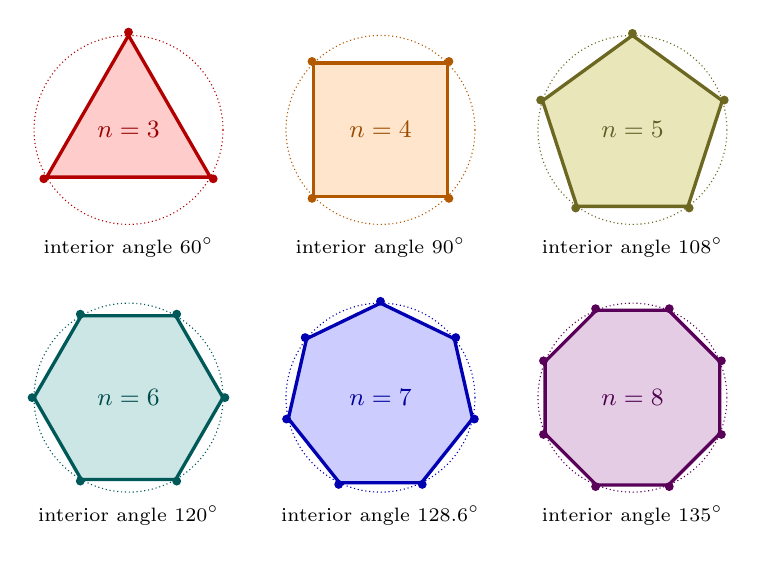
\begin{tikzpicture}
  \foreach \n/\c [count=\i from 0] in {3/red, 4/orange, 5/olive, 6/teal, 7/blue, 8/violet} {
    \pgfmathsetmacro\px{mod(\i,3)*3.2}
    \pgfmathsetmacro\py{-floor(\i/3)*3.4}
    \node[regular polygon, regular polygon sides=\n, minimum size=2.4cm, draw=\c!70!black,
          very thick, fill=\c!20] (p) at (\px,\py) {};
    \draw[\c!70!black, densely dotted] (\px,\py) circle (1.2cm);
    \foreach \k in {1,...,\n} { \fill[\c!70!black] (p.corner \k) circle (1.6pt); }
    \node[font=\small, \c!60!black] at (\px,\py) {$n=\n$};
    \pgfmathsetmacro\ang{180*(\n-2)/\n}
    \node[font=\scriptsize, below] at (\px,\py-1.25) {interior angle $\pgfmathprintnumber[precision=1]{\ang}^\circ$};
  }
\end{tikzpicture}
